% Sections/6_evaluation_results.tex
\section{Evaluation}
\subsection{Dataset Construction Engine Results}

The Dataset Construction Engine (DCE) effectiveness was tested by creating the UAVape dataset on it.

The final UAVape real dataset was built from two real-image batches. Batch A was the audited earlier real pool, while Batch B was the newly imported real-image batch used to evaluate the DCE's final intake, review, annotation and metadata workflow. The results therefore distinguish between the final combined dataset output and the Batch B workflow metrics used to test the DCE process.

Across the UAVape construction workflow, the DCE demonstrated its value as a dataset-construction engine rather than a narrow annotation interface. It supported real-image intake and audit through Batch B, produced a 2,905-image scraped source pool, generated 400 synthetic candidates and promoted 355 of them, assisted annotation through SAM2, populated metadata through VLM suggestions and exported a structurally valid YOLO dataset of 1,204 images and 2,040 boxes. These results establish that the DCE fulfilled its core role for SRQ1: converting fragmented micro-WEEE imagery into curated, annotated, metadata-enriched and model-ready data.


\subsubsection{End-to-End Source Construction}

The DCE-supported workflow produced a final combined real dataset from Batch A and Batch B, alongside two auxiliary training sources: scraped vape imagery and synthetic vape composites. The combined real dataset formed the official UAVape source of truth, while scraped and synthetic images were kept as source-separated training additions for later model ablation.

\begin{table}[H]
\centering
\small
\renewcommand{\arraystretch}{1.2}
\begin{tabularx}{\textwidth}{p{0.27\textwidth} r r X}
\toprule
\textbf{Source / output} & \textbf{Images} & \textbf{Boxes} & \textbf{Role in the DCE evaluation} \\
\midrule
Batch A real pool & 641 & 945 & Earlier audited real-image pool retained in the final dataset. \\
Batch B real pool & 563 & 1,095 & Newly imported real-image batch used to test the final DCE workflow. \\
Final combined real dataset & 1,204 & 2,040 & Human-reviewed real dataset constructed for detector training and evaluation. \\
Scraped vape training source & 2,905 & 4,437 & External source pool used to increase vape appearance diversity during training ablations. \\
Generated synthetic candidate pool & 400 & 400 & Synthetic composites generated by the DCE-controlled copy-paste pipeline. \\
Promoted synthetic training pool & 355 & 355 & Manually accepted synthetic composites eligible for source-controlled training use. \\
\bottomrule
\end{tabularx}
\caption{Source pools constructed or prepared through the DCE-supported dataset workflow.}
\label{tab:dce_results_source_construction}
\end{table}

This establishes the primary result for SRQ1: the DCE did not only label a pre-existing dataset, but supported the construction of multiple traceable source pools. Batch B was used as the main DCE workflow test batch, while the final combined real dataset contained 1,328 vape boxes and 712 lighter boxes. The scraped and synthetic sources were preserved separately so that their effect could be evaluated later in the model-ablation workstream.

\subsubsection{Multi-Source Intake and Scraping}

For real imagery, the largest logged direct-import batch was Batch B. This batch imported 574 images in approximately 0.35 minutes, giving a direct-import throughput of:

\begin{equation}
U_s = \frac{574}{0.35} = 1640 \text{ images/min}
\end{equation}

After manual audit, 563 of these 574 imported images remained active, meaning 11 images were rejected. Batch B is therefore used as the real-image workflow test case for the DCE results that follow.

\begin{table}[H]
\centering
\small
\renewcommand{\arraystretch}{1.2}
\begin{tabularx}{\textwidth}{p{0.34\textwidth} r X}
\toprule
\textbf{Intake / scrape metric} & \textbf{Value} & \textbf{Interpretation} \\
\midrule
Batch B images imported & 574 & Largest logged direct-import batch used in the final dataset build. \\
Direct-import time & 0.35 min & Elapsed import time from first to last logged import record. \\
Direct-import throughput, $U_s$ & 1640 images/min & Import-speed proxy for high-volume real-image intake. \\
Batch B images retained after audit & 563 & Active Batch B images after rejection of unusable images. \\
Batch B images rejected & 11 & Images removed during Batch B audit. \\
Exact duplicate hash groups & 0 & No exact duplicate groups in the current-real freeze. \\
Logged scraper development runs & 15 & Scraper runs preserved in the available development logs. \\
Logged scraper downloads & 5603 & Images downloaded across the preserved scraper logs. \\
Logged scraper failures & 402 & Download/process failures in the preserved scraper logs. \\
Logged duplicate skips & 1190 & Duplicate-source candidates intercepted in the preserved scraper logs. \\
Logged corrupt/too-small files & 45 & Corrupt or too-small files intercepted during scraper filtering. \\
\bottomrule
\end{tabularx}
\caption{Multi-source intake and scraper-log evidence from the DCE workflow.}
\label{tab:dce_results_intake_scraping}
\end{table}

The web scraper was used iteratively to build the dataset, ultimately sourcing 2,905 images containing 4,437 labelled vape boxes. Because the total number of raw, uncurated downloads was not tracked, an exact success rate cannot be calculated. Therefore, the scraper's value is measured by the usable data it produced rather than a formal efficiency benchmark.

\subsubsection{Synthetic Bootstrapping Yield}

The synthetic module was evaluated by comparing generated candidates with promoted candidates. A total of 400 synthetic images were generated, and 355 were manually promoted for training use. Using Equation~\ref{eq:synthetic_acceptance_rate}, this gives:

\begin{equation}
A_s = \frac{355}{400} \times 100 = 88.8\%
\end{equation}

\begin{table}[H]
\centering
\small
\renewcommand{\arraystretch}{1.2}
\begin{tabularx}{\textwidth}{p{0.34\textwidth} r X}
\toprule
\textbf{Synthetic metric} & \textbf{Value} & \textbf{Interpretation} \\
\midrule
Generated synthetic images & 400 & Full generated candidate pool. \\
Generated synthetic labels & 400 & Label files automatically produced for generated composites. \\
Promoted synthetic images & 355 & Manually accepted composites eligible for training use. \\
Promoted synthetic labels & 355 & Label files retained in the promoted synthetic pool. \\
Synthetic acceptance rate, $A_s$ & 88.8\% & Share of generated candidates promoted into the usable synthetic training pool. \\
\bottomrule
\end{tabularx}
\caption{Synthetic generation yield and manual promotion result.}
\label{tab:dce_results_synthetic}
\end{table}

This supports \textbf{DCE-DR2} because synthetic examples were generated as a separate candidate pool and only entered training after manual promotion. The 88.8\% acceptance rate indicates that the bounded controls produced a high proportion of usable composites. Rejections were primarily associated with unrealistic vape orientation, weak scene plausibility, or insufficient added visual diversity, showing that the promotion step acted as a quality-control filter rather than a simple bulk-generation process.

\subsubsection{Batch B Review Queue Throughput}

The Review Queue was evaluated using Batch B, the second real-image UAVape collection batch imported into the DCE. For this result, the metric of interest was not class balance, but how long it took to review a large newly imported batch inside the DCE.

Batch B contained 574 imported images. The logged review window ran for approximately 225.2 minutes, giving:

\begin{equation}
C_t = \frac{574}{225.2} = 2.55 \text{ images/min}
\end{equation}

This corresponds to approximately 23.5 seconds per image.

\begin{table}[H]
\centering
\small
\renewcommand{\arraystretch}{1.2}
\begin{tabularx}{\textwidth}{p{0.34\textwidth} r X}
\toprule
\textbf{Batch B review metric} & \textbf{Value} & \textbf{Interpretation} \\
\midrule
Batch B images reviewed & 574 & New real-image batch reviewed through the DCE. \\
Logged review window & 225.2 min & Approximate elapsed Review Queue period recorded for Batch B. \\
Curation throughput, $C_t$ & 2.55 images/min & Approximate Batch B review rate. \\
Mean review time per image & 23.5 s/image & Approximate time required to review each Batch B image. \\
\bottomrule
\end{tabularx}
\caption{Batch B Review Queue throughput inside the DCE.}
\label{tab:dce_results_curation}
\end{table}

This result supports DCE-DR3 by showing that the DCE could process a large real-image batch at a measurable review rate.

\subsubsection{Human-Audited SAM2 Annotation Performance}

SAM2 was evaluated as a human-audited proposal assistant. The DCE logs recorded 2,665 SAM2 proposals, which produced 2,040 accepted annotations in the final real dataset. This gives a proposal-to-accepted-annotation rate of 76.5\%. Among accepted annotations, 1,882 were first-click successes and 158 required at least one corrective re-click, giving:

\begin{equation}
FCA = \left(1 - \frac{158}{2040}\right) \times 100 = 92.3\%
\end{equation}

The cumulative corrective-click count was 337. Using Equation~\ref{eq:interaction_efficiency}, interaction efficiency was:

\begin{equation}
E = \frac{2040}{2040 + 337} \times 100 = 85.8\%
\end{equation}

\begin{table}[H]
\centering
\small
\renewcommand{\arraystretch}{1.2}
\begin{tabularx}{\textwidth}{p{0.34\textwidth} r X}
\toprule
\textbf{SAM2 metric} & \textbf{Value} & \textbf{Interpretation} \\
\midrule
SAM2 proposals generated & 2,665 & Draft masks/boxes requested through SAM2 mode. \\
Accepted annotations, $N$ & 2,040 & Final accepted annotations in the real dataset. \\
Proposal-to-annotation rate & 76.5\% & Share of generated proposals that became accepted annotations. \\
First-click successes & 1,882 & Accepted annotations requiring no corrective re-click. \\
Corrective re-click annotations, $N_{rc}$ & 158 & Accepted annotations requiring at least one corrective re-click. \\
First-click accuracy, $FCA$ & 92.3\% & Accepted annotations completed from the first click. \\
Cumulative corrective interactions, $R$ & 337 & Total corrective-click burden across accepted annotations. \\
Interaction efficiency, $E$ & 85.8\% & Finalised annotations relative to finalised plus corrective interactions. \\
Mean proposal accept time & 4.54 s & Event-level mean time from SAM2 proposal creation to human acceptance. \\
\bottomrule
\end{tabularx}
\caption{SAM2-assisted annotation efficiency and correction-burden metrics.}
\label{tab:dce_results_sam2}
\end{table}

A small retrospective manual baseline was also recorded by annotating 50 images with manual bounding boxes in Roboflow, producing a mean manual annotation time of 13.2 seconds per image. Compared with the SAM2 mean proposal accept time of 4.54 seconds, this gives an indicative time reduction of:

\begin{equation}
TR = \left(1 - \frac{4.54}{13.2}\right) \times 100 = 65.6\%
\end{equation}

This comparison supports the mechanical-efficiency claim of DCE-DR4, but should be interpreted as a small retrospective baseline rather than a full external usability study. The more robust logged evidence is the SAM2 interaction record itself: proposal counts, accept rates, first-click accuracy and corrective-interaction burden.

\subsubsection{VLM Metadata Reliability, Human Review and Coverage}

The metadata assistant was evaluated through three linked measures: VLM suggestion reliability, human correction activity and final metadata-field availability. Metadata was expected across the 2,040 accepted real-dataset annotations. Of these, 1,824 returned usable metadata suggestions and 216 failed or remained unusable. The VLM success rate was therefore:

\begin{equation}
\frac{1824}{2040} \times 100 = 89.4\%
\end{equation}

\begin{table}[H]
\centering
\small
\renewcommand{\arraystretch}{1.2}
\begin{tabularx}{\textwidth}{p{0.34\textwidth} r X}
\toprule
\textbf{VLM reliability metric} & \textbf{Value} & \textbf{Interpretation} \\
\midrule
Metadata suggestion attempts & 2,040 & Total expected metadata records across accepted real-dataset annotations. \\
Successful suggestions & 1,824 & VLM calls returning usable image-level metadata suggestions. \\
Failed suggestions & 216 & API failures or unusable suggestion outputs. \\
VLM success rate & 89.4\% & Overall reliability of the metadata assistant. \\
Human metadata correction records & 319 & Logged human edits to VLM-suggested metadata, showing that the assistant remained human-reviewed rather than automatically accepted. \\
\bottomrule
\end{tabularx}
\caption{VLM metadata suggestion reliability and human correction activity.}
\label{tab:dce_results_vlm_reliability}
\end{table}

The 319 correction records show where the human reviewer overrode the VLM most often. Object condition and viewpoint required the most correction, indicating that the VLM was more reliable at identifying visible scene properties such as clutter, blur and occlusion than it was at interpreting object state or camera angle.

\begin{table}[H]
\centering
\small
\renewcommand{\arraystretch}{1.2}
\begin{tabularx}{\textwidth}{p{0.30\textwidth} r X}
\toprule
\textbf{Metadata field corrected} & \textbf{Correction records} & \textbf{Interpretation} \\
\midrule
Object condition & 79 & Most frequently corrected; condition was visually ambiguous across damaged, wet or partially hidden objects. \\
Viewpoint & 63 & Camera angle often required human correction. \\
Lighting & 52 & Shadows and mixed illumination caused some VLM misclassification. \\
Surface & 47 & Ground-type labels sometimes required human correction. \\
Occlusion & 35 & Partial occlusion occasionally needed correction. \\
Background clutter & 28 & Generally reliable, but some clutter labels were adjusted. \\
Motion blur & 15 & Least corrected VLM-labelled field. \\
Scale band & 0 & Not corrected as a VLM field because it was calculated programmatically. \\
\bottomrule
\end{tabularx}
\caption{Human correction distribution across VLM-suggested metadata fields.}
\label{tab:dce_results_metadata_corrections}
\end{table}

Per-field metadata availability was then calculated after VLM suggestion, review and deterministic scale calculation. This table does not measure whether the original VLM suggestion was correct; it measures whether each field had a usable final value for later failure-mode analysis. Coverage was strongest for background clutter, occlusion and motion blur, while condition and viewpoint were weaker because those fields were more often left unknown or low-confidence.

\begin{table}[H]
\centering
\small
\renewcommand{\arraystretch}{1.2}
\begin{tabularx}{\textwidth}{p{0.30\textwidth} r X}
\toprule
\textbf{Metadata field} & \textbf{Coverage, $M_c$} & \textbf{Diagnostic value} \\
\midrule
Surface & 86.2\% & Enables surface-specific failure-mode analysis. \\
Lighting & 90.6\% & Enables illumination-specific error analysis. \\
Background clutter & 100.0\% & Supports analysis of visual-complexity effects. \\
Object condition & 42.5\% & Partially supports degradation/condition analysis. \\
Viewpoint & 44.5\% & Partially supports angle-specific analysis. \\
Occlusion & 99.9\% & Supports partial-visibility failure analysis. \\
Motion blur & 100.0\% & Supports blur-related deployment diagnostics. \\
Scale band & 100.0\% & Not produced by the VLM; calculated deterministically from bounding-box area after annotation. \\
\bottomrule
\end{tabularx}
\caption{Per-field metadata availability after VLM suggestion, human review and deterministic scale calculation.}
\label{tab:dce_results_metadata_coverage}
\end{table}

These results support DCE-DR5 by showing that the DCE could populate failure-mode metadata at scale while keeping the human reviewer in control. The correction records show that VLM outputs were treated as suggestions rather than ground truth, and the per-field availability table shows which metadata dimensions were strongest for downstream failure-mode analysis. Scale band is not interpreted as a VLM field because the method deliberately treats scale as a deterministic geometry-derived value.

\subsubsection{COCO Source of Truth and YOLO Export Readiness}

The final stage of the DCE workflow was export readiness. The high-resolution COCO source of truth retained 2,040 annotations across two classes: \texttt{vape} and \texttt{lighter}. The final active YOLO export contained 1,204 images, 1,204 label files and 2,040 boxes, with zero export warnings.

This satisfies DCE-DR6. The DCE preserved a COCO source of truth for annotation integrity while producing a lightweight YOLO dataset suitable for the downstream detector benchmark. The final output of the DCE was therefore not only a set of labelled images, but a traceable, model-ready dataset with source labels, metadata, class IDs and export manifests.

\subsection{UAVape Model Results}

The detector-selection benchmark compared YOLO26, YOLO11 and YOLOv8 families across model scale and input resolution. Table~\ref{tab:uavape_results_detector_selection_main} reports the full 16-run validation benchmark using both aggregate two-class metrics and vape-specific metrics. Aggregate mAP is retained for transparency, but vape AP is the target-class metric because disposable vapes are the primary research object and lighters are an auxiliary confuser class.

\begin{table}[H]
\centering
\scriptsize
\resizebox{\textwidth}{!}{%
\begin{tabular}{r l r r r r r}
\toprule
\textbf{Rank} & \textbf{Run} & \textbf{Best epoch} & \textbf{All mAP@50} & \textbf{All mAP@50--95} & \textbf{Vape AP50} & \textbf{Vape AP50--95} \\
\midrule
\textbf{1} & \textbf{YOLO26s @ 1280} & \textbf{77} & \textbf{0.80233} & \textbf{0.60501} & \textbf{0.91763} & \textbf{0.70669} \\
2 & YOLO11s @ 1280 & 74 & 0.78559 & 0.58851 & 0.87978 & 0.67722 \\
\textbf{3} & \textbf{YOLO11s @ 960} & \textbf{89} & \textbf{0.77487} & \textbf{0.56639} & \textbf{0.90301} & \textbf{0.67675} \\
\textbf{4} & \textbf{YOLO26m @ 640} & \textbf{82} & \textbf{0.79481} & \textbf{0.56215} & \textbf{0.88876} & \textbf{0.66603} \\
5 & YOLO26s @ 960 & 90 & 0.74253 & 0.54957 & 0.85692 & 0.68355 \\
6 & YOLO11n @ 960 & 90 & 0.76500 & 0.54500 & 0.87800 & 0.64500 \\
7 & YOLOv8s @ 1280 & 76 & 0.73735 & 0.54448 & 0.80318 & 0.61764 \\
8 & YOLO26s @ 640 & 71 & 0.76095 & 0.54024 & 0.87651 & 0.64776 \\
9 & YOLOv8s @ 960 & 89 & 0.73797 & 0.53573 & 0.86633 & 0.65877 \\
10 & YOLOv8m @ 640 & 88 & 0.75316 & 0.53368 & 0.87318 & 0.64843 \\
11 & YOLO26n @ 960 & 78 & 0.72900 & 0.52700 & 0.83500 & 0.63300 \\
12 & YOLO11m @ 640 & 81 & 0.75816 & 0.52415 & 0.88178 & 0.64840 \\
13 & YOLO11s @ 640 & 87 & 0.74736 & 0.50696 & 0.89317 & 0.63779 \\
14 & YOLOv8s @ 640 & 69 & 0.71935 & 0.48731 & 0.83862 & 0.59569 \\
15 & YOLO26n @ 640 & 74 & 0.68700 & 0.45900 & 0.82900 & 0.59800 \\
16 & YOLO11n @ 640 & 89 & 0.68800 & 0.45600 & 0.85300 & 0.58700 \\
\bottomrule
\end{tabular}}
\caption{Full detector-selection validation benchmark. Bold rows indicate the selected 1280-pixel protocol and the strongest lower-resolution comparator rows used to interpret deployment trade-offs.}
\label{tab:uavape_results_detector_selection_main}
\end{table}

The benchmark selected YOLO26s at 1280 pixels because it led both the aggregate ranking and the vape-class ranking. However, the lower-resolution results were still promising: YOLO26m at 640 reached vape AP50 of 0.889 and vape AP50--95 of 0.666, while YOLO11s at 960 reached vape AP50 of 0.903 and aggregate mAP@50--95 of 0.566. This means that the final 1280-pixel model should be read as the strongest accuracy protocol, while 640- and 960-pixel variants remain plausible candidates for future edge-hardware testing.

\subsubsection{SAHI Tiling Validation Branch}

SAHI-style tiled inference was tested as a validation-only branch on the lower pixel models. The aim was to improve their performance to match or outperform the 1280px models. However, tiling worsened these models. The tiled runs produced a very high number of predictions relative to the 302 effective validation instances, suggesting that duplicate detections, tile-boundary effects or false-positive pressure outweighed any benefit from increased local detail.

\begin{table}[H]
\centering
\scriptsize
\resizebox{\textwidth}{!}{%
\begin{tabular}{l r r r r r r r}
\toprule
\textbf{Run} & \textbf{Predictions} & \textbf{All AP50} & \textbf{All AP50--95} & \textbf{Vape AP50} & \textbf{Vape AP50--95} & \textbf{Lighter AP50} & \textbf{Lighter AP50--95} \\
\midrule
YOLO26s @ 640 + SAHI 1280/20\% & 9131 & 0.63982 & 0.48436 & 0.72741 & 0.55774 & 0.55223 & 0.41098 \\
YOLO26s @ 960 + SAHI 1280/20\% & 7568 & 0.69592 & 0.51027 & 0.80554 & 0.60559 & 0.58631 & 0.41494 \\
YOLO11s @ 960 + SAHI 1280/20\% & 10449 & 0.68078 & 0.51124 & 0.76595 & 0.58479 & 0.59561 & 0.43769 \\
YOLO11n @ 960 + SAHI 1280/20\% & 14250 & 0.67804 & 0.50773 & 0.75871 & 0.56937 & 0.59736 & 0.44609 \\
\bottomrule
\end{tabular}}
\caption{Full SAHI-style tiled inference validation results.}
\label{tab:uavape_results_sahi_main}
\end{table}

\subsubsection{Data-Source Ablation}

The data-source ablation was thereby tested on the benchmark YOLO26s model at 1280px. The aim was to test whether source-controlled scraped and synthetic vape imagery improved validation performance. Table~\ref{tab:uavape_results_ablation_main} combines the training recipe and key validation metrics so the effect of each source addition can be read directly.

\begin{table}[H]
\centering
\scriptsize
\resizebox{\textwidth}{!}{%
\begin{tabular}{l l r r r r r}
\toprule
\textbf{Run} & \textbf{Training recipe} & \textbf{Train images} & \textbf{All AP50} & \textbf{All AP50--95} & \textbf{Vape AP50} & \textbf{Vape AP50--95} \\
\midrule
\texttt{A0\_real\_only} & V4 real train only & 837 & 0.802 & 0.605 & 0.918 & 0.707 \\
\texttt{S88\_scraped} & V4 real + 88 scraped & 925 & 0.774 & 0.601 & 0.874 & 0.696 \\
\texttt{S177\_scraped} & V4 real + 177 scraped & 1014 & 0.799 & 0.619 & 0.899 & 0.720 \\
\texttt{S355\_scraped} & V4 real + 355 scraped & 1192 & 0.777 & 0.611 & 0.891 & 0.718 \\
\texttt{Y88\_synthetic} & V4 real + 88 synthetic & 925 & 0.803 & 0.617 & 0.912 & 0.712 \\
\texttt{Y177\_synthetic} & V4 real + 177 synthetic & 1014 & 0.792 & 0.598 & 0.903 & 0.692 \\
\texttt{Y355\_synthetic} & V4 real + 355 synthetic & 1192 & 0.793 & 0.616 & 0.898 & 0.716 \\
\texttt{S355\_Y355\_combined} & V4 real + 355 scraped + 355 synthetic & 1547 & 0.815 & 0.639 & 0.922 & 0.737 \\
\bottomrule
\end{tabular}}
\caption{Validation results from the V4 data-source ablation under the fixed YOLO26s@1280 protocol.}
\label{tab:uavape_results_ablation_main}
\end{table}

The combined scraped-plus-synthetic recipe produced the strongest validation result, improving vape AP50 from 0.918 to 0.922 and vape AP50--95 from 0.707 to 0.737 relative to the real-only baseline. The scraped-only and synthetic-only branches were mixed and non-monotonic, so the result supports a source-mixture conclusion rather than a simple ``more data is always better'' conclusion.

\subsubsection{Final Sealed Test Result}

After validation-based selection, the \texttt{S355\_Y355\_combined} \texttt{best.pt} checkpoint was evaluated once on the sealed real-image test split. Table~\ref{tab:uavape_results_final_test_main} reports the selected validation result and the final held-out test result.

\begin{table}[H]
\centering
\scriptsize
\resizebox{\textwidth}{!}{%
\begin{tabular}{l r r r r r r r r r r}
\toprule
\textbf{Split} & \textbf{Images} & \textbf{Instances} & \textbf{All P} & \textbf{All R} & \textbf{All AP50} & \textbf{All AP50--95} & \textbf{Vape AP50} & \textbf{Vape AP50--95} & \textbf{Lighter AP50} & \textbf{Lighter AP50--95} \\
\midrule
Validation & 183 & 302 & 0.833 & 0.774 & 0.815 & 0.639 & 0.922 & 0.737 & 0.708 & 0.541 \\
Test & 184 & 420 & 0.849 & 0.725 & 0.851 & 0.638 & 0.882 & 0.685 & 0.819 & 0.591 \\
\bottomrule
\end{tabular}}
\caption{Validation and sealed test results for the selected \texttt{S355\_Y355\_combined} recipe.}
\label{tab:uavape_results_final_test_main}
\end{table}

On the sealed test split, the selected detector achieved all-class mAP@50 of 0.851 and mAP@50--95 of 0.638. The target vape class reached AP50 of 0.882 and AP50--95 of 0.685. The validation vape AP50 of 0.922 should therefore be interpreted as selection evidence, while the test vape AP50 of 0.882 is the final held-out generalisation score.

\subsubsection{Selected Detector Properties}

\begin{table}[H]
\centering
\small
\begin{tabularx}{\textwidth}{p{0.30\textwidth} X}
\toprule
\textbf{Property} & \textbf{Selected detector value} \\
\midrule
Detector checkpoint & YOLO26s \texttt{best.pt} from the \texttt{S355\_Y355\_combined} run \\
Input size & 1280 pixels, full-frame inference \\
Parameter count & 9,465,954 parameters \\
Compute estimate & 20.5 GFLOPs \\
Final-test runtime environment & RunPod H100 NVL, Ultralytics 8.4.62 \\
\bottomrule
\end{tabularx}
\caption{Deployment-relevant properties recorded for the selected detector. Server-GPU timing is reported for transparency but does not represent UAV edge-hardware performance.}
\label{tab:uavape_results_selected_detector_deployment_properties_main}
\end{table}

\subsection{Cleaner Workflow Evaluation}

\subsubsection{Prototype Output}

The cleaner workflow prototype was implemented as a clickable HTML wireframe pack titled \textit{UAVape Cleanup Planner}. The prototype translated vape detections into task-based information: evidence crops, map points, confidence scores, hazard labels, task assignment and field status updates. The prototype was not connected to live UAV detections or a municipal backend. It was evaluated as a workflow concept.

\begin{figure}[H]
    \centering
    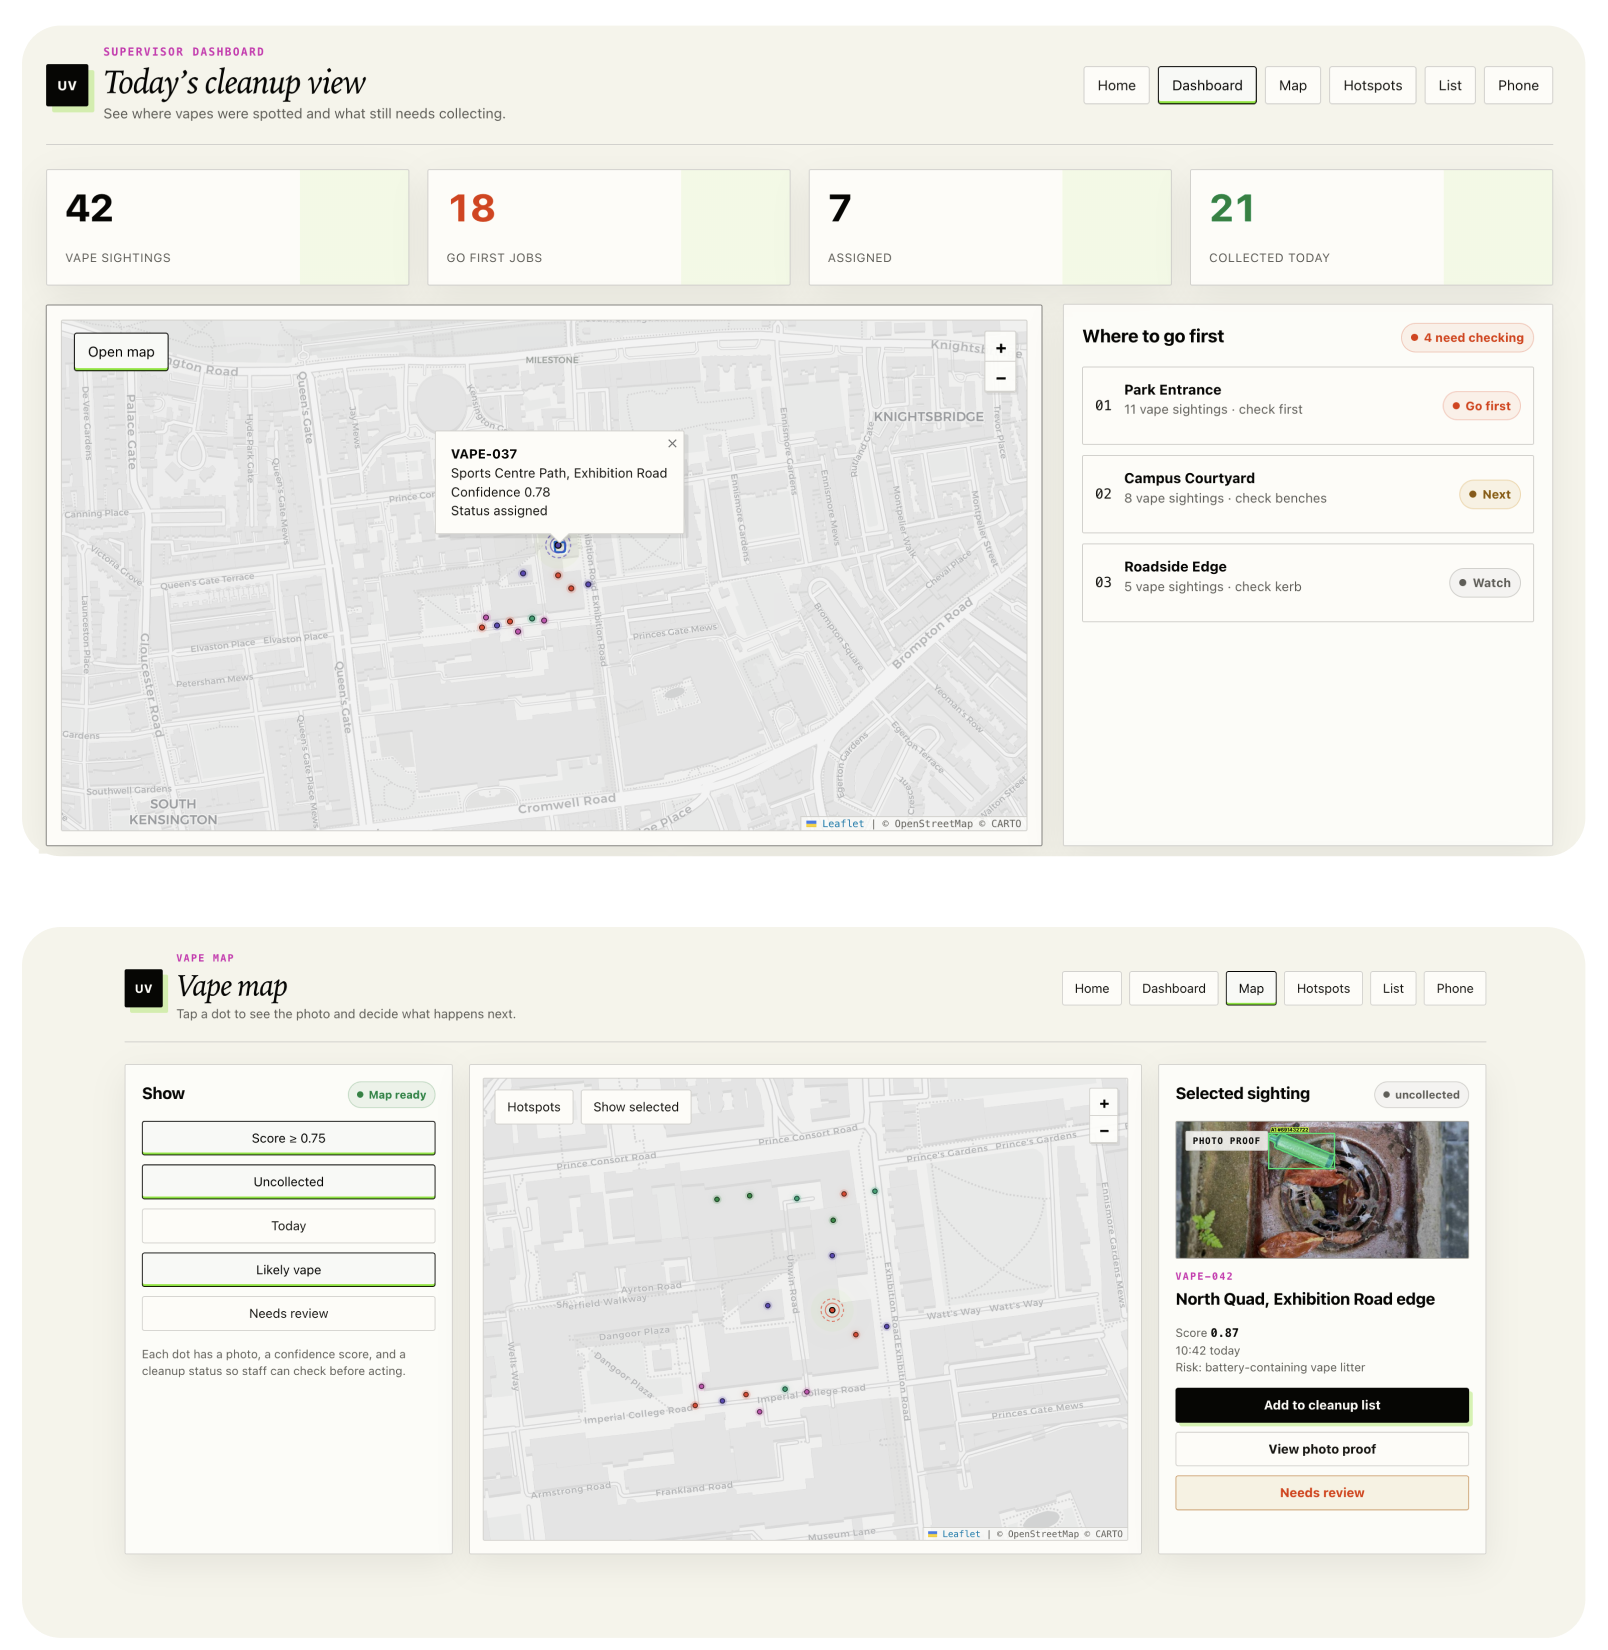
\includegraphics[width=0.7\linewidth]{Supervisor Interface.png}
    \caption{Clean-up planning interfaces}
    \label{fig:supervisor_interface}
\end{figure}

\begin{figure}[H]
    \centering
    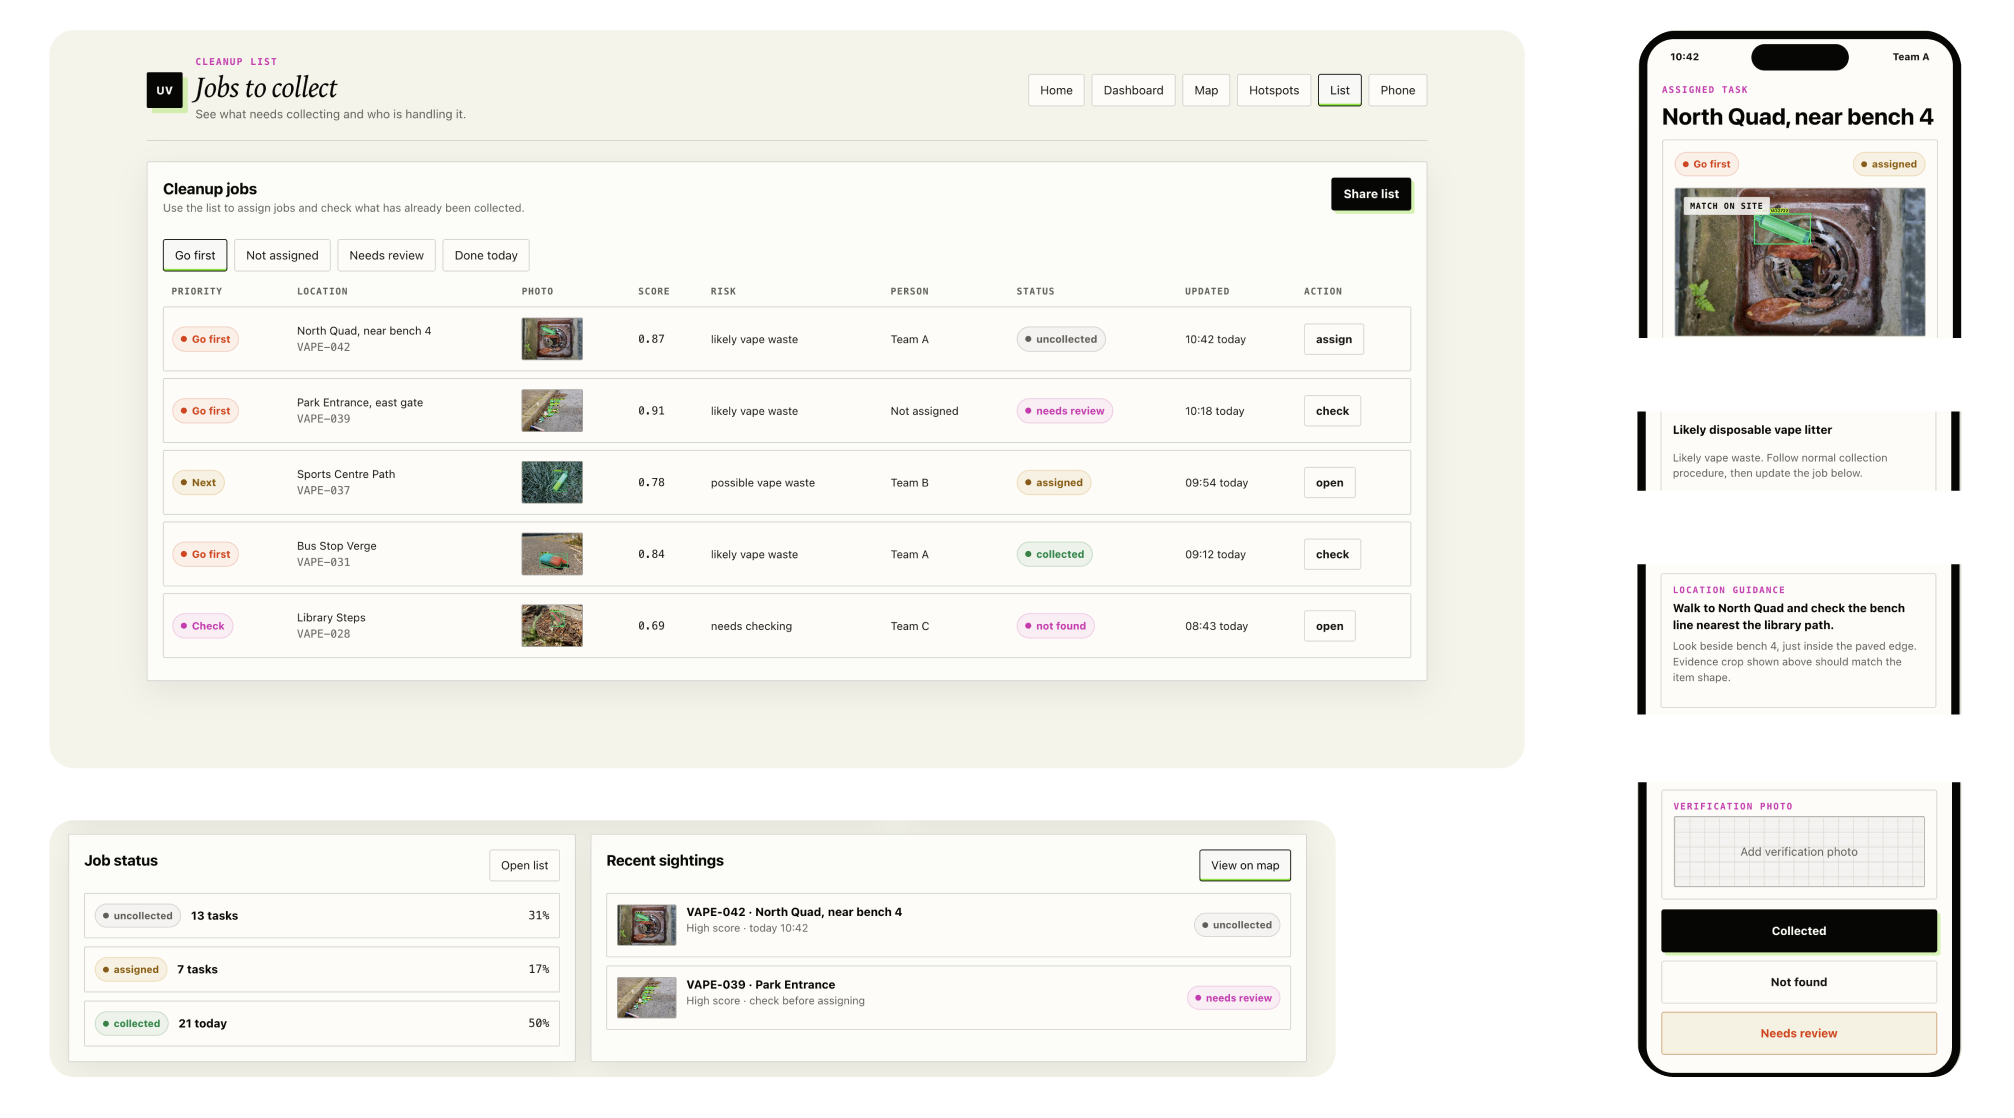
\includegraphics[width=0.7\linewidth]{Cleaner Interface.png}
    \caption{Cleaner-tasking interfaces}
    \label{fig:cleaner_interface}
\end{figure}

\subsubsection{Stakeholder Survey Findings}

\begin{figure}[H]
    \centering
    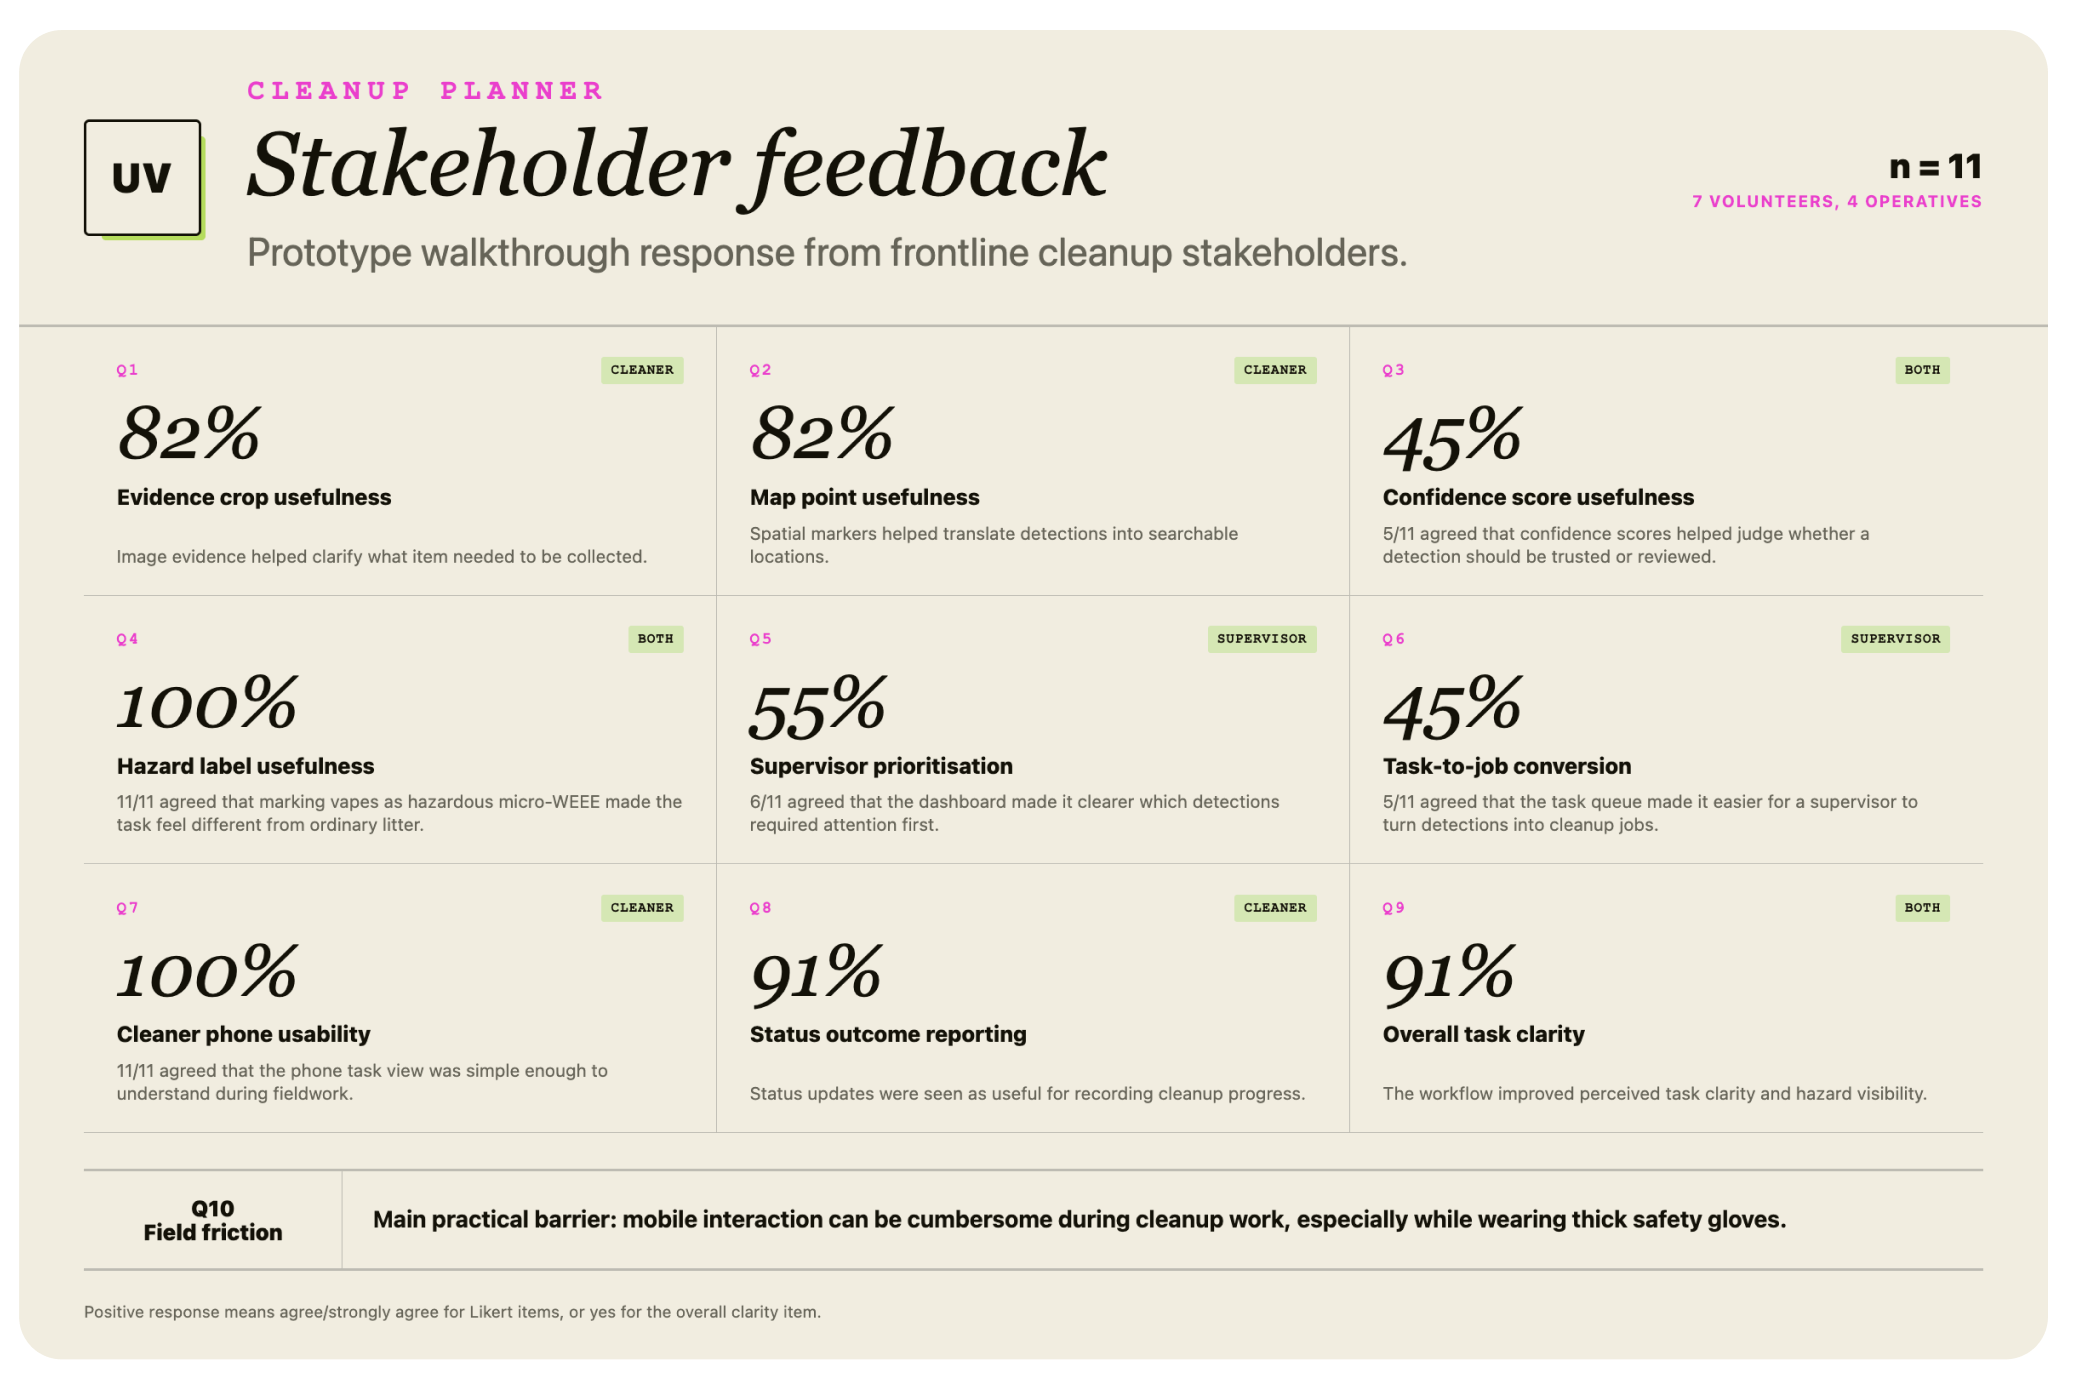
\includegraphics[width=0.7\linewidth]{UIRES.png}
    \caption{Stakeholder feedback on the UAVape Cleanup Planner prototype.}
    \label{fig:cleaner_feedback_infographic}
\end{figure}

The walkthrough was completed with 11 frontline stakeholders. The strongest result was hazard communication: 11 of 11 participants responded positively to labelling disposable vapes as hazardous micro-WEEE. This supports the decision to keep vape detections separate from generic litter in the interface.

Evidence and location support were also received positively. Nine of 11 participants agreed that evidence crops and map points helped clarify what needed to be collected and where it was located. Status reporting and overall workflow clarity were each supported by 10 of 11 participants. This suggests that the prototype made the detection-to-cleanup process easier to understand than a purely manual or route-based workflow.

The lower-scoring items were confidence score usefulness, supervisor prioritisation and task-to-job conversion. This suggests that participants understood the field-facing parts of the workflow more easily than the supervisory planning layer. This is expected because the walkthrough group consisted mainly of frontline cleaners and volunteers rather than municipal supervisors.

The open-text response identified one practical field constraint: using a phone interface can be difficult during cleanup work, especially when wearing thick safety gloves. Future versions should therefore use larger touch targets, fewer status actions or alternative input methods such as voice. These findings should be interpreted as prototype feedback, not evidence of full municipal deployment readiness.

\vspace{1em}
\noindent \textbf{$\hookrightarrow$ Design Requirements Met (Cleaner Workflow UI): UI-DR1, UI-DR2, UI-DR3, UI-DR4}
